\section{Supuestos}
	A continuación se hace mención de los requerimientos necesarios para iniciar la instalación.
	\begin{itemize}
		\item Sistema operativo Debian GNU/Linux 7 whezzy.
		\item Tener actualizado los repositorios.
		\item Deshabilitar el DHCP del router a utilizar (módem en su defecto).
		\item Habilitar la Ip estática tanto en el servidor como en el módem.
	\end{itemize}		
	
\section{Instalación del ISC DHCP}
En Debian GNU/Linux, el paquete de software que contiene el servidor DHCP de ISC (Internet System Consortium) se denomina isc-dhcp-server y para su instalación procedemos de la siguiente manera:
	
	\begin{listing}[style=consola, numbers=none]
	    $  apt-get install isc-dhcp-server
 	\end{listing}

	Una vez instalado, como podemos ver a continuación, se intenta automáticamente lanzar el servidor pero da un fallo debido a que aún no hay ninguna configuración establecida.
	
	\begin{listing}[style=consola, numbers=none]
	    $  	isc-dhcp-server, action "start" failed.
 	\end{listing}

El programa que implementa el servidor DHCP es /usr/sbin/dhcpd y éste, como todos los servicios, lo podremos manejar a través de un script del directorio /etc/init.d/ o bien con el comando service:

	\begin{listing}[style=consola, numbers=none]
# /etc/init.d/isc-dhcp-server
Usage: /etc/init.d/isc-dhcp-server {start|stop|restart|force-reload|status}
# /etc/init.d/isc-dhcp-server start
[ ok ] Starting ISC DHCP server: dhcpd.
 	\end{listing}

La instalación anterior del servidor debe haber configurado el sistema operativo para que se active automáticamente cuando se encienda el ordenador. Esto lo podemos comprobar mirando que exista el fichero que lanzará el arranque (Start) del servidor DHCP, el cual debe encontrarse al menos en el directorio init del nivel de arranque actual de nuestro sistema operativo. Para saber cuál es el nivel de arranque actual usaremos la instrucción who:

	\begin{listing}[style=consola, numbers=none]
	$ who -r
	$ ls /etc/rc2.d
 	\end{listing}
	
	Como resultado se debe encontrar el archivo S17isc-dhcp-server, con ello aseguramos que se inicie al reiniciar el servidor.\\

Ficheros del servidor DHCP a tener en cuenta son los siguientes:
	\begin{itemize}
		\item /etc/dhcp/dhcpd.conf: es el fichero de configuración del servidor. Se puede modificar con el servidor ejecutándose, y una vez modificado reiniciaremos el servicio.
		\item /var/lib/dhcp/dhcpd.leases: es el fichero base de datos donde se registran todas las concesiones de IP que se van dando a los clientes.
		\item /etc/default/isc-dhcp-server: desde aquí se puede especificar qué ficheros sustituirán a los dos anteriores; también, cuáles serán las interfaces por las que el servidor DHCP escuchará peticiones de IP.
		\item /var/log/syslog: en este fichero se irán escribiendo los mensajes log del servidor DHCP, a menos que lo cambiemos a otro fichero.
		\item /var/run/dhcpd.pid: contiene el PID de servidor DHCP (dhcpd).
		\item /usr/share/doc/isc-dhcp-*: varios directorios donde hay diversa documentación sobre el servicio DHCP junto con ejemplos.
	\end{itemize}		

Podemos usar la orden man para obtener diversa documentación:

	\begin{itemize}
		\item man dhcpd
		\item man dhcpd.conf
		\item man dhcp-options
		\item man dhcp-eval
	\end{itemize}		

\subsection{/etc/default/isc-dhcp-server}
El fichero /etc/default/isc-dhcp-server es el primer fichero de configuración que lee el servidor DHCP (/usr/sbin/dhcpd), y con él podemos cambiar varias cosas que veremos a continuación.

A veces el ordenador donde se encuentra el servidor DHCP tiene más de una interfaz de red, y puede que necesitemos que éste no trabaje por todas las interfaces, es decir, que sólo atienda peticiones por unas cuantas. Para hacer esto debemos modificar la variable INTERFACES. El valor por defecto es el siguiente:

	\begin{listing}[style=texto, numbers=none]
	INTERFACES=""
 	\end{listing}

lo cual indica que el servidor escucha peticiones por todas sus interfaces. Si sólo debe escuchar por las interfaz eth0, pondríamos el siguiente valor:
	\begin{listing}[style=texto, numbers=none]
	INTERFACES="eth0"
 	\end{listing}
 	
 	
%\begin{figure}
%  \centering
%    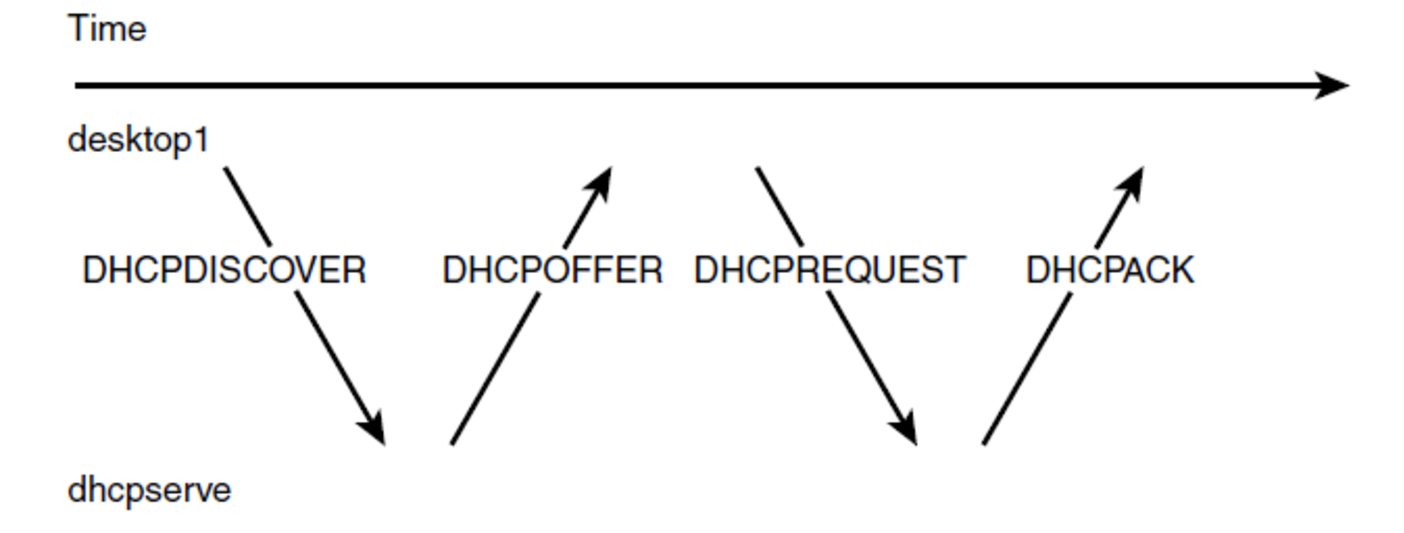
\includegraphics[width=0.7\textwidth]{img/com}
%  \caption{Dos servidores}
%  \label{fig:3}
%\end{figure}



%\begin{listing}[style=consola, numbers=none]
%	    $ cd ~/Downloads/
% \end{listing}



%%%%%%%%%% Ejemplo de una tabla %%	
	
%	\begin{table}[h]
%\centering
%\begin{tabular}{l|c|c|c}
%\hline\hline \rowcolor{LightBlue2} Factor a analizar& Peso relativo &Calificación&Calificación ponderada\\ \hline\hline
%\multicolumn{4}{c}{FORTALEZAS}\\ \hline
%F-1& 0.2 		& 4& 0.8 \\
%F-2 & 0.15 & 4& 0.6 \\
%F-3 & 0.1 	& 2&  0.2\\
%F-4 & 0.1 	& 2&  0.2\\
%F-5 & 0.15 & 3&  0.45\\
%F-6 & 0.05 & 2&  0.1\\\hline
%\multicolumn{3}{r}{Total}& 2.35\\ \hline
%\multicolumn{4}{c}{DEBILIDADES}\\ \hline
%D-1& 0.15 & 3& 0.45\\
%D-2 & 0.10 & 2& 0.2\\\hline
%Total&1 & & 0.65\\ \hline
%\end{tabular}
%\caption{MEFI}
%\end{table}